\documentclass[a4paper, 12pt]{article}

\usepackage[utf8]{inputenc}
\usepackage{amsmath}
\usepackage[]{amsfonts}
\usepackage[]{graphicx}

\title{CS231A Course Notes 3: Epipolar Geometry}
\author{Kenji Hata and Silvio Savarese}
\date{}


\renewcommand\emph{\textbf}

\begin{document}

\maketitle

\section{Introduction}
Previously, we have seen how to compute the intrinsic and extrinsic parameters of a camera using one or more views using a typical camera calibration procedure or single view metrology. This process culminated in deriving properties about the 3D world from one image. However, in general, it is not possible to recover the entire structure of the 3D world from just one image. This is due to the intrinsic ambiguity of the 3D to the 2D mapping: some information is simply lost.

\begin{figure}[h!]
\centering

\includegraphics[width=0.8\textwidth]{figures/pisa.jpg}
\caption{A single picture such as this picture of a man holding up the Leaning Tower of Pisa can result in ambiguous scenarios. Multiple views of the same scene help us resolve these potential ambiguities.}
\label{fig:pisa}
\end{figure}

For example, in Figure~\ref{fig:pisa}, we may be initially fooled to believe that the man is holding up the Leaning Tower of Pisa. Only by careful inspection can we tell that this is not the case and merely an illusion based on the projection of different depths onto the image plane. However, if we were able to view this scene from a completely different angle, this illusion immediately disappears and we would instantly figure out the correct scene layout. 

The focus of these lecture notes is to show how having knowledge of geometry when multiple cameras are present can be extremely helpful. Specifically, we will first focus on defining the geometry involved in two viewpoints and then present how this geometry can aid in further understanding the world around us. 

\section{Epipolar Geometry}
\begin{figure}[h!]
\centering
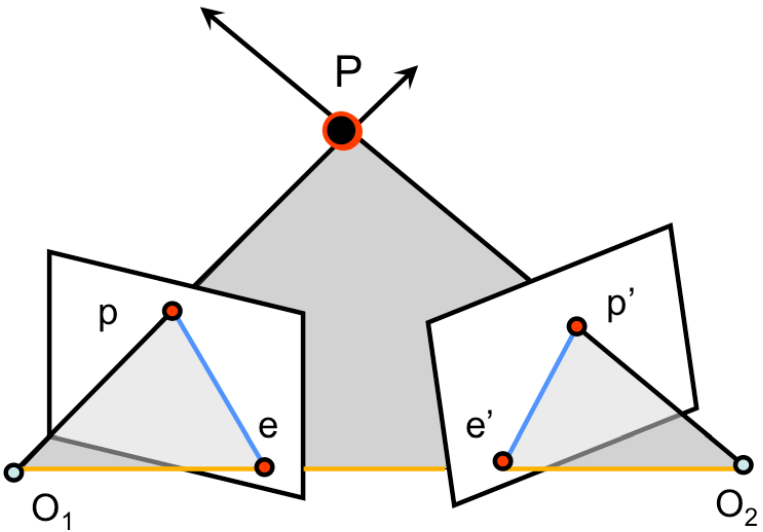
\includegraphics[width=0.8\textwidth]{figures/epipolar.png}
\caption{The general setup of epipolar geometry. The gray region is the epipolar plane. The orange line is the baseline, while the two blue lines are the epipolar lines.}
\label{fig:epipolar}
\end{figure}
Often in multiple view geometry, there are interesting relationships between the multiple cameras, a 3D point, and that point's projections in each of the camera's image plane. The geometry that relates the cameras, points in 3D, and the the corresponding observations is referred to as the \emph{epipolar geometry} of a stereo pair. 

\begin{figure}[h!]
\centering
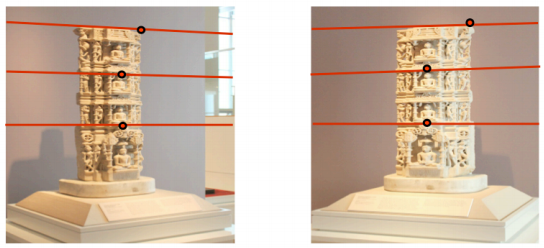
\includegraphics[width=0.8\textwidth]{figures/epipolar_example.png}
\caption{An example of epipolar lines and their corresponding points drawn on an image pair.}
\label{fig:epipolar_example}
\end{figure}
As illustrated in Figure~\ref{fig:epipolar}, the standard epipolar geometry setup involves two cameras observing the same 3D point $P$, whose projection in each of the image planes is located at $p$ and $p'$ respectively. The camera centers are located at $O_1$ and $O_2$, and the line between them is referred to as the \emph{baseline}. We call the plane defined by the two camera centers and $P$ the \emph{epipolar plane}. The locations of where the baseline intersects the two image planes are known as the the \emph{epipoles} $e$ and $e'$. Finally, the lines defined by the intersection of the epipolar plane and the two image planes are known as the \emph{epipolar lines}. The epipolar lines have the property that they intersect the baseline at the respective epipoles in the image  plane.

\begin{figure}[h!]
\centering
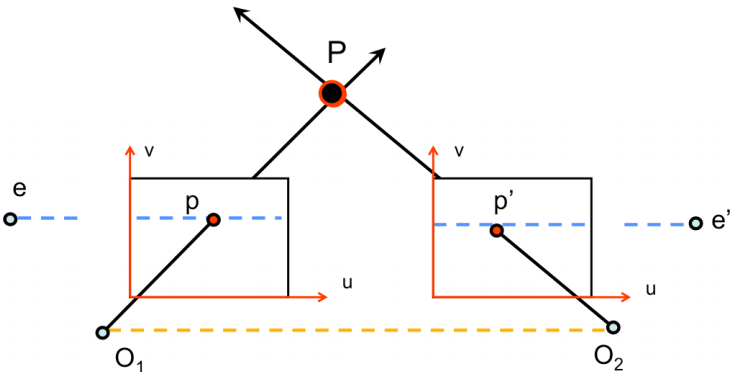
\includegraphics[width=0.8\textwidth]{figures/epipolar_parallel.png}
\caption{When the two image planes are parallel, then the epipoles $e$ and $e'$ are located at infinity. Notice that the epipolar lines are parallel to the $u$ axis of each image plane.}
\label{fig:epipolar_parallel}
\end{figure}

An interesting case of epipolar geometry is shown in Figure~\ref{fig:epipolar_parallel}, which occurs when the image planes are parallel to each other. When the image planes are parallel to each other, then the epipoles $e$ and $e'$ will be located at infinity since the baseline joining the centers $O_1,O_2$ is parallel to the image planes. Another important byproduct of this case is that the epipolar lines are parallel to an axis of each image plane. This case is especially useful and will be covered in greater detail in the subsequent section on image rectification.

In real world situations, however, we are not given the exact location of the 3D location $P$, but can determine its projection in one of the image planes $p$. We also should be able to know the cameras locations, orientations, and camera matrices. What can we do with this knowledge? With the knowledge of camera locations $O_1, O_2$ and the image point $p$, we can define the epipolar plane. With this epipolar plane, we can then determine the epipolar lines\footnote{This means that epipolar lines can be determined by just knowing the camera centers $O_1, O_2$ and a point in one of the images $p$}. By definition, $P$'s projection into the second image $p'$ must be located on the epipolar line of the second image. Thus, a  basic understanding of epipolar geometry allows us to create a strong constraint between image pairs without knowing the 3D structure of the scene. 

\begin{figure}[h!]
\centering
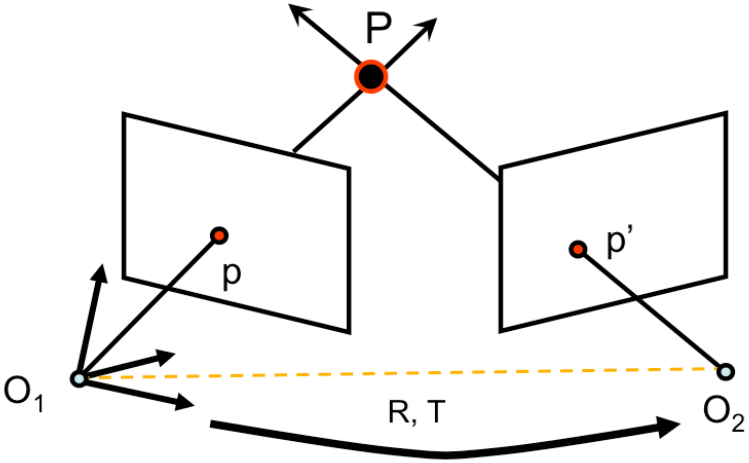
\includegraphics[width=0.8\textwidth]{figures/essential_fundamental_setup.png}
\caption{The setup for determining the essential and fundamental matrices, which help map points and epipolar lines across views.}
\label{fig:essential_fundamental_setup}
\end{figure}

We will now try to develop seamless ways to do map points and epipolar lines across views. If we take the setup given in the original epipolar geometry framework (Figure~\ref{fig:essential_fundamental_setup}), then we shall further define $M$ and $M'$ to be the camera projection matrices that map 3D points into their respective 2D image plane locations. Let us assume that the world reference system is associated to the first camera with the second camera offset first by a rotation $R$ and then by a translation $T$. This specifies the camera projection matrices to be:
\begin{equation}
    M = K\begin{bmatrix} I & 0\end{bmatrix} \ \ \ \ \ M' = K'\begin{bmatrix}R & T\end{bmatrix}
    \label{eq:projection_matrices}
\end{equation}

\section{The Essential Matrix}
In the simplest case, let us assume that we have \emph{canonical cameras}, in which $K = K' = I$. This reduces Equation~\ref{eq:projection_matrices} to 

\begin{equation}
    M = \begin{bmatrix} I & 0\end{bmatrix} \ \ \ \ \ M' = \begin{bmatrix}R & T\end{bmatrix}
    \label{eq:projection_matrices_canonical}
\end{equation}

Furthermore, this means that the location of $p'$ in the first camera's reference system is $R^Tp' - R^TT$. Since the vectors $R^Tp' - R^TT$ and $R^TT$ lie in the epipolar plane, then if we take the cross product of $R^TT\times(R^Tp' -R^T T) = R^TT \times R^Tp' = R^T(T \times p')$, we will get a vector normal to the epipolar plane. This also means that $p$, which lies in the epipolar plane is normal to $R^T(T\times p')$, giving us the constraint that their dot product is zero:
\begin{equation}
    \begin{split}
    	(R^T(T\times p')))^T p = 0\\
    	(T\times p')^T R p = 0 \\ 
    \end{split}
    \label{eq:essential1}
\end{equation}

From linear algebra, we can introduce a different and compact expression for the cross product: we can represent the cross product between any two vectors $a$ and $b$ as a matrix-vector multiplication:
\begin{equation}
    \mathbf{a}\times \mathbf{b} = \begin{bmatrix} 0 & -\mathbf{a}_z & \mathbf{a}_y \\ \mathbf{a}_z & 0 & -\mathbf{a}_x \\ -\mathbf{a}_y & \mathbf{a}_x & 0\end{bmatrix}\begin{bmatrix} \mathbf{b}_x \\ \mathbf{b}_y \\ \mathbf{b}_z\end{bmatrix} = [\mathbf{a}_\times] \mathbf{b}
\end{equation}

Combining this expression with Equation~\ref{eq:essential1}, we can convert the cross product term into matrix multiplication, giving
\begin{equation}
    \begin{split}
        ([T_\times] p')^T R p = 0 \\ 
    	  p'^T [T_\times]^T R p = 0 \\
	  p'^T [T_\times] R p = 0
    \end{split}
\end{equation}
The matrix $E = [T_\times]R$ is known as the \emph{Essential Matrix}, creating a compact expression for the epipolar constraint: 
\begin{equation}
    p'^T E p = 0
\end{equation}
The Essential matrix is a $3\times3$ matrix that contains 5 degrees of freedom. It has rank 2 and is singular. 

The Essential matrix is useful for computing the epipolar lines associated with $p$ and $p'$. For instance, $\ell' = Ep$ gives the epipolar line in the image of camera 2. Similarly $\ell = E^Tp'$ gives the epipolar line in the image of camera 1. Other interesting properties of the essential matrix is that its matrix product with the epipoles equate to zero: $Ee = E^Te' = 0$. 
%TODO: WHY???

%TODO: Section on deriving the Rotation and Translation from E  

\section{The Fundamental Matrix}
Although, we derived a relationship between $p$ and $p'$ when we have canonical cameras, we should be able to find a more general expression when the cameras are no longer canonical. Recall that gives us the projection matrices:

\begin{equation}
    M = K\begin{bmatrix} I & 0\end{bmatrix} \ \ \ \ \ M' = K'\begin{bmatrix}R & T\end{bmatrix}
    \label{eq:projection_matrices2}
\end{equation}

First, we must define $p_c = K^{-1}p$ and $p_c' = K'^{-1}p'$ to be the projections of $P$ to the corresponding camera images if the cameras were canonical. Recall that in the canonical case:
\begin{equation}
    p'^T_c [T_\times]Rp_c = 0
    \label{eq:canonical_constraint}
\end{equation}
By substituting in the values of $p_c$ and $p_c'$, we get
\begin{equation}
    p'^TK^{-T} [T_\times]RK'^{-1}p = 0
    \label{eq:canonical_constraint_substitute}
\end{equation}
The matrix $F = K^{-T} [T_\times]RK'^{-1}$ is known as the \emph{Fundamental Matrix}, which acts similar to the Essential matrix from the previous section but also encodes information about the camera matrices $K, K'$ and the relative translation $T$ and rotation $R$ between the cameras. Therefore, it is also useful in computing the epipolar lines associated with $p$ and $p'$, even when the camera matrices $K, K'$ and the transformation $R,T$ are unknown. Similar to the Essential matrix, we can compute the epipolar lines $\ell' = Fp$ and $\ell = F^T p'$ from just the Fundamental matrix and the corresponding points. One main difference between the Fundamental matrix and the Essential matrix is that the Fundamental matrix contains 7 degrees of freedom, compared to the Essential matrix's 5 degrees of freedom.

But how is the Fundamental matrix useful? Like the Essential matrix, if we know the Fundamental matrix, then simply knowing a point in an image gives us an easy constraint (the epipolar line) of the corresponding point in the other image. Therefore, without knowing the actual position of $P$ in 3D space, or any of the extrinsic or intrinsic characteristics of the cameras, we can establish a relationship between any $p$ and $p'$. 

\begin{figure}[h!]
\centering
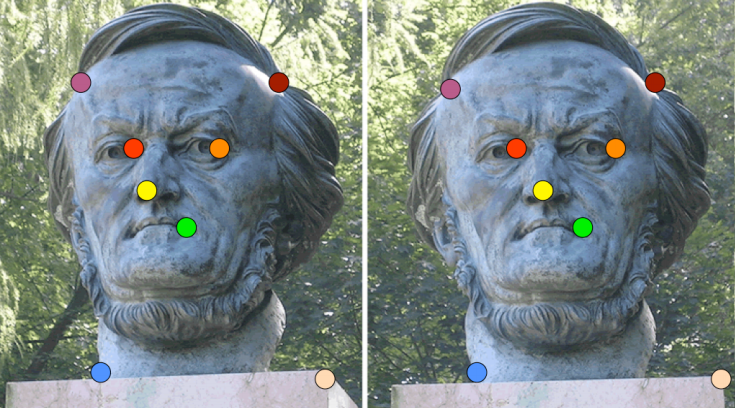
\includegraphics[width=0.8\textwidth]{figures/correspondence.png}
\caption{Corresponding points are drawn in the same color on each of the respective images.}
\label{fig:correspondence}
\end{figure}

\subsection{The Eight-Point Algorithm}
Still, the assumption that we can have the Fundamental matrix, which is defined by a matrix product of the camera parameters, seems rather large. However, it is possible to estimate the Fundamental matrix given two images of the same scene and without knowing the extrinsic or intrinsic parameters of the camera. The method we discuss for doing so is known as the \emph{Eight-Point Algorithm}, which was proposed by Longuet-Higgins in 1981 and extended by Hartley in 1995. As the title suggests, the Eight-Point Algorithm assumes that a set of at least 8 pairs of corresponding points between two images is available.

Each correspondence $p_i = (u_i, v_i, 1)$ and $p'_i = (u_i', v_i', 1)$ gives us the epipolar constraint $p_i'^T F p_i = 0$. We can reformulate the constraint as follows:
\begin{equation}
    \begin{bmatrix}u_iu_i' & v_iu_i' & u'_i & u_iv'_i &  v_iv_i' & v_i' & u_i & v_i & 1\end{bmatrix}
    \begin{bmatrix}F_{11}\\F_{12}\\F_{13}\\F_{21}\\F_{22}\\F_{23}\\F_{31}\\F_{32}\\F_{33}\end{bmatrix} = 0
\end{equation}

Since this constraint is a scalar equation, it only constrains one degree of freedom. Since we can only know the Fundamental matrix up to scale, we require eight of these constraints to determine the Fundamental matrix:

\begin{equation}
    \begin{bmatrix}
    u_1u_1' & v_1u_1' & u'_1 & u_1v'_1 &  v_1v_1' & v_1' & u_1 & v_1 & 1 \\ 
    u_2u_2' & v_2u_2' & u'_2 & u_2v'_2 &  v_2v_2' & v_2' & u_2 & v_2 & 1 \\
    u_3u_3' & v_3u_3' & u'_3 & u_3v'_3 &  v_3v_3' & v_3' & u_3 & v_3 & 1 \\
    u_4u_4' & v_4u_4' & u'_4 & u_4v'_4 &  v_4v_4' & v_4' & u_4 & v_4 & 1\\
    u_5u_5' & v_5u_5' & u'_5 & u_5v'_5 &  v_5v_5' & v_5' & u_5 & v_5 & 1\\
    u_6u_6' & v_6u_6' & u'_6 & u_6v'_6 &  v_6v_6' & v_6' & u_6 & v_6 & 1 \\
    u_7u_7' & v_7u_7' & u'_7 & u_7v'_7 &  v_7v_7' & v_7' & u_7 & v_7 & 1 \\
    u_8u_8' & v_8u_8' & u'_8 & u_8v'_8 &  v_8v_8' & v_8' & u_8 & v_8 & 1
    \end{bmatrix}
    \begin{bmatrix}F_{11}\\F_{12}\\F_{13}\\F_{21}\\F_{22}\\F_{23}\\F_{31}\\F_{32}\\F_{33}\end{bmatrix} = 0
\end{equation}
This can be compactly written as 
\begin{equation}
    W\mathbf{f} = 0
    \label{eq:compact_8}
\end{equation}
where $W$ is an $N\times 9$ matrix derived from $N \geq 8$ correspondences and $\mathbf{f}$ is the values of the Fundamental matrix we desire. 

In practice, it often is better to use more than eight correspondences and create a larger $W$ matrix because it reduces the effects of noisy measurements. The solution to this system of homogeneous equations can be found in the least-squares sense by Singular Value Decomposition (SVD), as $W$ is rank-deficient. SVD will give us a estimate of the Fundamental matrix $\hat{F}$, which may have full rank. However, we know that the true Fundamental matrix has rank 2. Therefore, we should look for a solution that is the best rank-2 approximation of $\hat{F}$. To do so, we solve the following optimization problem:
\begin{equation}
\begin{aligned}
& \underset{F}{\text{minimize}}
& & \|F-\hat{F}\|_\mathrm{F}  \\
& \text{subject to}
& & \det F = 0
\end{aligned}
\end{equation}
This problem is solved again by SVD, where $\hat{F} = U\Sigma V^T$, then the best rank-2 approximation is found by
\begin{equation}
F = U\begin{bmatrix}\Sigma_1&0&0\\0&\Sigma_2&0\\0&0&0\end{bmatrix}V^T
\end{equation}

\subsection{The Normalized Eight-Point Algorithm}
In practice, the standard least-squares approach to the Eight-Point Algorithm is not precise. Often, the distance between a point $p_i$ and its corresponding epipolar line $\ell_i = F^Tp'$ will be very large, usually on the scale of 10+ pixels. To reduce this error, we can consider a modified version of the Eight-Point Algorithm called the \emph{Normalized Eight-Point Algorithm}. 

The main problem of the standard Eight-Point Algorithm stems from the fact that $W$ is ill-conditioned for SVD. For SVD to work properly, $W$ should have one singular value equal to (or near) zero, with the other singular values being nonzero. However, the correspondences $p_i = (u_i, v_i, 1)$ will often have extremely large values in the first and second coordinates due to the pixel range of a modern camera (i.e. $p_i = (1832, 1023, 1))$. If the image points used to construct $W$ are in a relatively small region of the image, then each the vectors for $p_i$ and $p_i'$ will generally be very similar. Consequently, the constructed $W$ matrix will have one very large singular value, with the rest relatively small. 

To solve this problem, we will normalize the points in the image before constructing $W$. This means we \emph{pre-condition} $W$ by applying both a translation and scaling on the image coordinates such that two requirements are satisfied. First, the origin of the new coordinate system should be located at the centroid of the image points (translation). Second, the mean square distance of the transformed image points from the origin should be 2 pixels (scaling). We can compactly represent this process by a transformation matrices $T, T'$ that translate by the centroid and scale by the scaling factor $\frac{2}{\mathrm{mean\ distance}}$ for each respective image.

Afterwards, we normalize the coordinates:
\begin{equation}
q_i = Tp_i \ \ \ \ \ q_i' = T'p_i'
\end{equation}
Using the new, normalized coordinates, we can compute the new $F_q$ using the regular least-squares Eight Point Algorithm. However, the matrix $F_q$ is the fundamental matrix for the normalized coordinates. For it to be usable on regular coordinate space, we need to de-normalize it, giving
\begin{equation}
F = T'^TF_qT
\end{equation}
Ultimately, this new Fundamental matrix $F$ gives good results in real-world applications.

\section{Image Rectification}

Recall that an interesting case for epipolar geometry occurs when two images are parallel to each other. Let us first compute the Essential matrix $E$ in the case of parallel image planes. We can assume that the two cameras have the same $K$ and that there is no relative rotation between the cameras ($R= I$. In this case, let us assume that there is only a translation along the $x$ axis, giving $T = (T_x, 0, 0)$. This gives
\begin{equation}
E = [T_\times] R = \begin{bmatrix} 0 & 0 & 0\\ 0 & 0 & -T_x \\ 0 & T_x  & 0 \end{bmatrix}
\end{equation}

Once $E$ is known, we can find the directions of the epipolar lines associated with points in the image planes. Let us compute the direction of the epipolar line $\ell$ associated with point $p'$:
\begin{equation}
\ell = Ep' = \begin{bmatrix} 0 & 0 & 0\\ 0 & 0 & -T_x \\ 0 & T_x  & 0 \end{bmatrix} \begin{bmatrix}u'\\v'\\1\end{bmatrix} = \begin{bmatrix} 0\\ -T \\ Tv'\end{bmatrix}
\end{equation}
We can see that the direction of $\ell$ is horizontal, as is the direction of $\ell'$, which is computed in a similar manner.
\begin{figure}[h!]
\centering
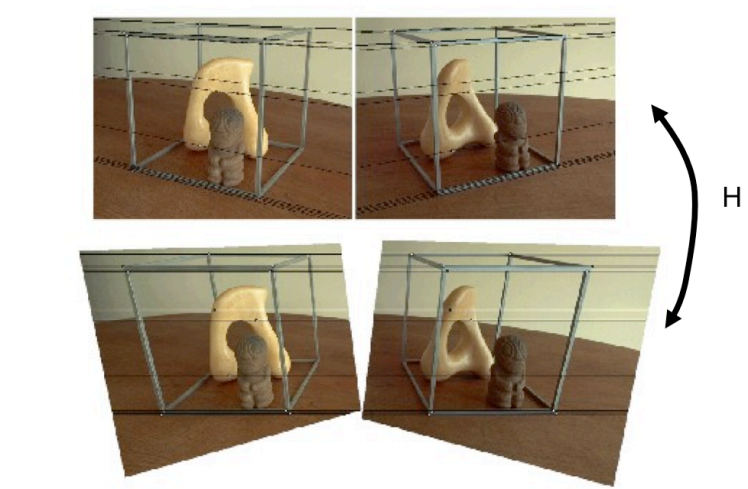
\includegraphics[width=0.8\textwidth]{figures/rectification_example.png}
\caption{The process of image rectification involves computing two homographies that we can apply to a pair of images to make them parallel.}
\label{fig:rectification_example}
\end{figure}
 

If we use the epipolar constraint $p'^T Ep=0$, then we arrive at the fact that $v=v'$, demonstrating that $p$ and $p'$ share the same $v$-coordinate. Consequently, there exists a very straightforward relationship between the corresponding points. Therefore, \emph{rectification}, or the process of making any two given images parallel, becomes useful when discerning the relationships between corresponding points in images.

\begin{figure}[h!]
\centering
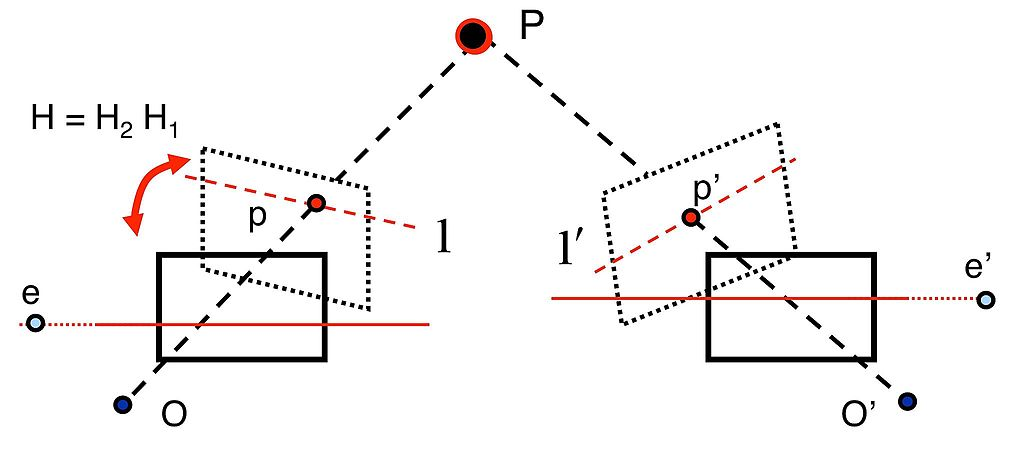
\includegraphics[width=0.8\textwidth]{figures/rectification_setup.jpg}
\caption{The rectification problem setup: we compute two homographies that we can apply to the image planes to make the resulting planes parallel.}
\label{fig:rectification_setup}
\end{figure}

Rectifying a pair of images does not require knowledge of the two camera matrices $K, K'$ or the relative transformation $R,T$ between them. Instead, we can use the Fundamental matrix estimated by the Normalized Eight Point Algorithm. Upon getting the Fundamental matrix, we can compute the epipolar lines $\ell_i$ and $\ell_i'$ for each correspondence $p_i$ and $p_i'$. 

From the set of epipolar lines, we can then estimate the epipoles $e$ and $e'$ of each image. This is because we know that the epipole lies in the intersection of all the epipolar lines. In the real world, due to noisy measurements, all the epipolar lines will not intersect in a single point. Therefore, computing the epipole can be found by minimizing the least squared error of fitting a point to all the epipolar lines. Recall that each epipolar line can be represented as a vector $\ell$ such that all points on the line (represented in homogeneous coordinates) are in the set $\{x | \ell^Tx = 0\}$. If we define each epipolar line as $\ell_i = \begin{bmatrix}\ell_{i,1} & \ell_{i,2} & \ell_{i,3} \end{bmatrix}^T$, then we can we formulate a linear system of equations and solve using SVD to find the epipole $e$:
\begin{equation} 
    \begin{bmatrix}
    \ell_{1}^T\\
    \vdots\\
    \ell_{n}^T
    \end{bmatrix}e = 0
\end{equation}

After finding the epipoles $e$ and $e'$, we will most likely notice that they are not points at infinity along the horizontal axis. If they were, then, by definition, the images would already be parallel. Thus, we gain some insight into how to make the images parallel: can we find a homography to map an epipole $e$ to infinity along the horizontal axis? Specifically, this means that we want to find a pair of homographies $H_1, H_2$ that we can apply to the images to map the epipoles to infinity. Let us start by finding a homography $H_2$ that maps the second epipole $e'$ to a  point on the horizontal axis at infinity $(f,0,0)$. Since there are many possible choices for this homography, we should try to choose something reasonable. One condition that leads to good results in practice is to insist that the homography acts like a transformation that applies a translation and rotation on points near the center of the image. 

The first step in achieving such a transformation is to translate the second image such that the center is at $(0,0,1)$ in homogeneous coordinates. We can do so by applying the translation matrix
\begin{equation}
    T = \begin{bmatrix}
    1&0&-\frac{\mathrm{width}}{2}\\0&1&-\frac{\mathrm{height}}{2}\\ 0 &0 &1
    \end{bmatrix}
\end{equation}
After applying the translation, we apply a rotation to place the epipole on the horizontal axis at some point $(f,0,1)$. If the translated epipole $Te'$ is located at homogeneous coordinates $(e'_1, e'_2, 1)$, then the rotation applied is
\begin{equation}
    R = 
    \begin{bmatrix}
        \alpha\frac{e'_1}{\sqrt{e_1'^2+e_2'^2}} & \alpha\frac{e'_2}{\sqrt{e_1'^2+e_2'^2}} & 0 \\ -\alpha\frac{e'_2}{\sqrt{e_1'^2+e_2'^2}} &\alpha \frac{e'_1}{\sqrt{e_1'^2+e_2'^2}} & 0\\ 0&0&1
    \end{bmatrix}
\end{equation}
where $\alpha=1$ if $e'_1\geq 0$ and $\alpha=-1$ otherwise. After applying this rotation, notice that given any point at $(f,0,1)$, bringing it to a point at infinity on the horizontal axis $(f,0,0)$ only requires applying a transformation
\begin{equation}
    G =
    \begin{bmatrix}
    1 & 0 &0 \\ 0 & 1 & 0 \\ -\frac{1}{f} & 0 & 1
    \end{bmatrix}
\end{equation}
After applying this transformation, we finally have an epipole at infinity, so we can translate back to the regular image space. Thus, the homography $H_2$ that we apply on the second image to rectify it is 
\begin{equation}
    H_2 = T^{-1}GRT 
\end{equation}

Now that a valid $H_2$ is found, we need to find a matching homography $H_1$ for the first image. We do so by finding a transformation $H_1$ that minimizes the sum of square distances between the corresponding points of the images
\begin{equation}
    \arg \min_{H_1} \sum_i \|H_1p_i - H_2 p_i'\|^2 
    \label{eq:rectification_minimization}
\end{equation}
Although the derivation\footnote{If you are interested in the details, please see Chapter 11 of Hartley \& Zisserman's textbook \textit{Multiple View Geometry}} is outside the scope of this class, we can actually prove that the matching $H_1$ is of the form:
\begin{equation}
    H_1 = H_A H_2 M
\label{eq:matching_homography}
\end{equation}
where $F= [e]_\times M$ and
\begin{equation}
    H_A = \begin{bmatrix} a_1 & a_2 & a_3\\ 0 & 1 & 0 \\ 0 & 0 &1\end{bmatrix}
\end{equation}
with $(a_1, a_2, a_3)$ composing the elements of a certain vector $\mathbf{a}$ that will be computed later. 

First, we need to know what $M$ is. An interesting property of any $3\times3$ skew-symmetric matrix $A$ is $A = A^3$ up to scale. Because any cross product matrix $[e]_\times$ is skew-symmetric and that we can only know the Fundamental matrix $F$ up to scale, then 
\begin{equation}
    F = [e]_\times M = [e]_\times [e]_\times [e]_\times M = [e]_\times [e]_\times F
\end{equation}
By grouping the right terms, we can find that 
\begin{equation}
    M = [e]_\times F
\end{equation}
Notice that if the columns of $M$ were added by any scalar multiple of $e$, then the $F = [e]_\times M$ still holds up to scale. Therefore, the more general case of defining $M$ is
\begin{equation}
    M = [e]_\times F + e v^T
\end{equation}
for some vector $v$. In practice, defining $M$ by setting $v=\begin{bmatrix}1 & 1 & 1\end{bmatrix}$ works very well.

To finally solve for $H_1$, we need to compute the $\mathbf{a}$ values of $H_A$. Recall that we want to find a $H_1, H_2$ to minimize the problem posed in Equation~\ref{eq:rectification_minimization}. Since we already know the value of $H_2$ and $M$, then we can substitute $\hat{p}_i = H_2Mp_i$ and $\hat{p}_i' = H_2p_i'$ and the minimization problem becomes
\begin{equation}
\arg \min_{H_A} \sum_i \|H_A\hat{p}_i - \hat{p}_i'\|^2 
\end{equation}

In particular, if we let $\hat{p}_i = (\hat{x}_i, \hat{y}_i, 1)$ and $\hat{p}_i' = (\hat{x}_i', \hat{y}_i', 1)$, then the minimization problem can be replaced by:
\begin{equation}
\arg \min_{\mathbf{a}} \sum_i (a_1\hat{x}_i + a_2\hat{y}_i + a_3 - \hat{x}_i')^2 + (\hat{y}_i -\hat{y}_i')^2 
\end{equation}
Since $\hat{y}_i -\hat{y}_i'$ is a constant value, the minimization problem further reduces to
\begin{equation}
\arg \min_{\mathbf{a}} \sum_i (a_1\hat{x}_i + a_2\hat{y}_i + a_3 - \hat{x}_i')^2
\end{equation}

Ultimately, this breaks down into solving a least-squares problem $W\mathbf{a} = b$ for $\mathbf{a}$ where
\begin{equation}
W = \begin{bmatrix} \hat{x}_1 & \hat{y}_1 & 1 \\ &\vdots& \\ \hat{x}_n & \hat{y}_n & 1 \end{bmatrix} \ \ \ \ \ \ b = \begin{bmatrix}\hat{x}_1' \\ \vdots \\ \hat{x}_n'\end{bmatrix}
\end{equation}

After computing $\mathbf{a}$, we can compute $H_A$ and finally $H_1$. Thus, we generated the homographies $H_1,H_2$ to rectify any image pair given a few correspondences.
\end{document}
